\chapter{Interfaz del simulador y alojamiento web}
\par En este capítulo se describe la interfaz gráfica diseñada para interactuar con el simulador, consistente en pantallas de introducción de datos y pantallas para mostrar los resultados del simulador. Adicionalmente, se describe la plataforma usada para alojar el simulador en la web.

\section{Interfaz de usuario (UI)}
\par Una interfaz de usuario (UI, abreviación comúnmente usada en inglés) es el medio por el cual una persona interactúa con una aplicación de software o dispositivo de hardware. Esto significa que el programa incluye controles gráficos que optimizan la experiencia de usuario usando un ratón, teclado o pantalla táctil.
\par Los elementos más comunes de una interfaz gráfica de usuario, de acuerdo con Career Foundry \cite{ui}, son:
\begin{itemize}
\item Controles de entrada: permiten introducir información en el sistema por parte de los usuarios.
\item Componentes de navegación: ayudan a los usuarios a moverse.
\item Componentes informativos: brindan información a los usuarios.
\item Contenedores: mantienen el contenido organizado, como paneles, ventanas, marcos, etc.
\end{itemize}
\par Sin la interfaz de usuario, el algoritmo, aunque poderoso, tendría un uso muy limitado por la complejidad que implica correrlo directamente como un programa y por lo difícil que es observar los cambios sin una amigable visualización de datos.
\par La interfaz de usuario implementada para el algoritmo se desarrolló usando los lenguajes básicos de desarrollo web: Lenguaje de Marcado de Hipertexto (HTML), Hojas de Estilo en Cascada (CSS) y el lenguaje de programación interpretado JavaScript (JS), lo que hace que sea totalmente editable y pueda correr en cualquier ordenador o dispositivo móvil con navegador web sin instalar otro programa. 
\par La interfaz desarrollada consiste en un sitio web donde el usuario puede navegar a distintas vistas con diferentes propósitos. A continuación se describirán dichas vistas y sus aplicaciones pensadas, esencialmente las posibilidades educativas que ofrece la comparación de dos estados del proceso, pero no limitadas a estas.

\subsection{Descripción de uso y alcances}
\par Al ingresar al enlace del simulador, la vista de bienvenida otorga instrucciones y limitaciones de uso del simulador, al ser la vista principal el usuario podrá conocer todas las capacidades y aplicaciones disponibles en la versión actual publicada (ver la Figura \ref{fig:alcance}).
\par Aquí se describen las condiciones de operación de diseño establecidas para dar una referencia al usuario de las cargas que puede manejar el horno simulado dentro de los rangos sugeridos de uso.
\begin{figure}[H]
\begin{center}
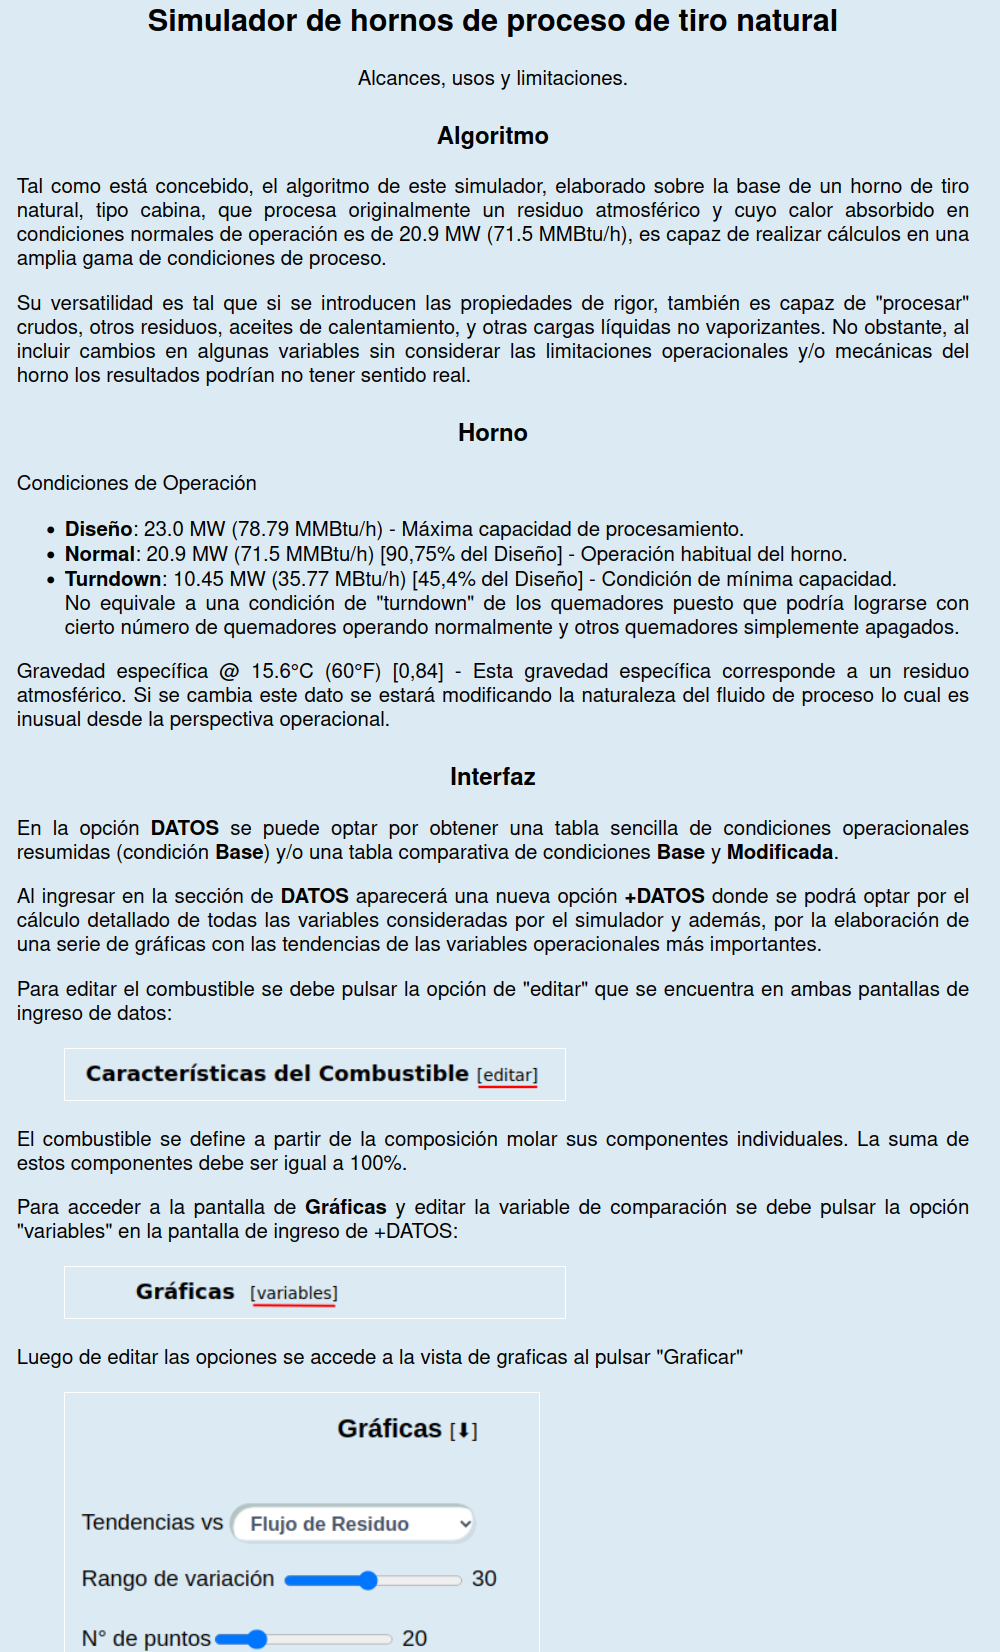
\includegraphics[scale=0.33]{images/alcance}
\caption[Página de alcances]{Referencia a página de alcances, vista introductoria a la aplicación web.}
\label{fig:alcance}
\end{center}
\end{figure}
\par La sección de usos y alcance describe como utilizar la barra de navegación del sitio web (ver Figura \ref{fig:navbar}), como editar el combustible a utilizar en las diferentes vistas de ingreso de datos y finalmente como usar la sección de gráficas o tendencias.
\begin{figure}[H]
\begin{center}

\includegraphics[scale=0.22]{images/navbar}
\caption[Barra de navegación]{Barra de navegación de la interfaz web.}
\label{fig:navbar}
\end{center}
\end{figure}

\subsubsection{Condiciones de operación de diseño}
\par En esta vista se detallan las condiciones de diseño, como se muestra a continuación:
\begin{itemize}
    \item \textbf{Diseño}: 23.0 MW (78.79 MMBtu/h) - Máxima capacidad de procesamiento recomendada.
    \item \textbf{Normal}: 20.9 MW (71.5 MMBtu/h) [90,75\% del Diseño] - Operación habitual del horno.
    \item \textbf{Turndown}*: 10.45 MW (35.77 MBtu/h) [45,4\% del Diseño] - Condición mínima de operación.
\end{itemize}
\par *No equivale a una condición de ``turndown'' de los quemadores puesto que podría lograrse con cierto número de quemadores operando normalmente y otros quemadores simplemente apagados.

\subsection{Introducción de datos}
\par En esta sección se desarrollan dos vistas:
\begin{itemize}
    \item La primera, que se accede al pulsar el botón \textbf{DATOS} en la barra de navegación, es una vista simplificada para introducir solo los datos más relevantes del proceso. Al accionar el cálculo dirige al usuario a una pantalla de resultados donde se pueden comparar dos estados de operación (ver Fig. \ref{fig:datos}).
    \item La segunda, que se accede estando en la sección de ingreso de datos simplificada al pulsar el botón \textbf{+DATOS} en la barra de navegación. En esta vista se encuentran todas las variables que permite modificar el proceso (ver Fig. \ref{fig:fulldatos}) y permite la posibilidad de accionar el cálculo para ofrecer una página de resultados extendidos. Adicionalmente se pueden accionar la generación de las curvas de tendencia escogiendo una variable a ser modificada al final de la página y pulsando el botón de graficar.
\end{itemize}
\begin{figure}[H]
\begin{center}
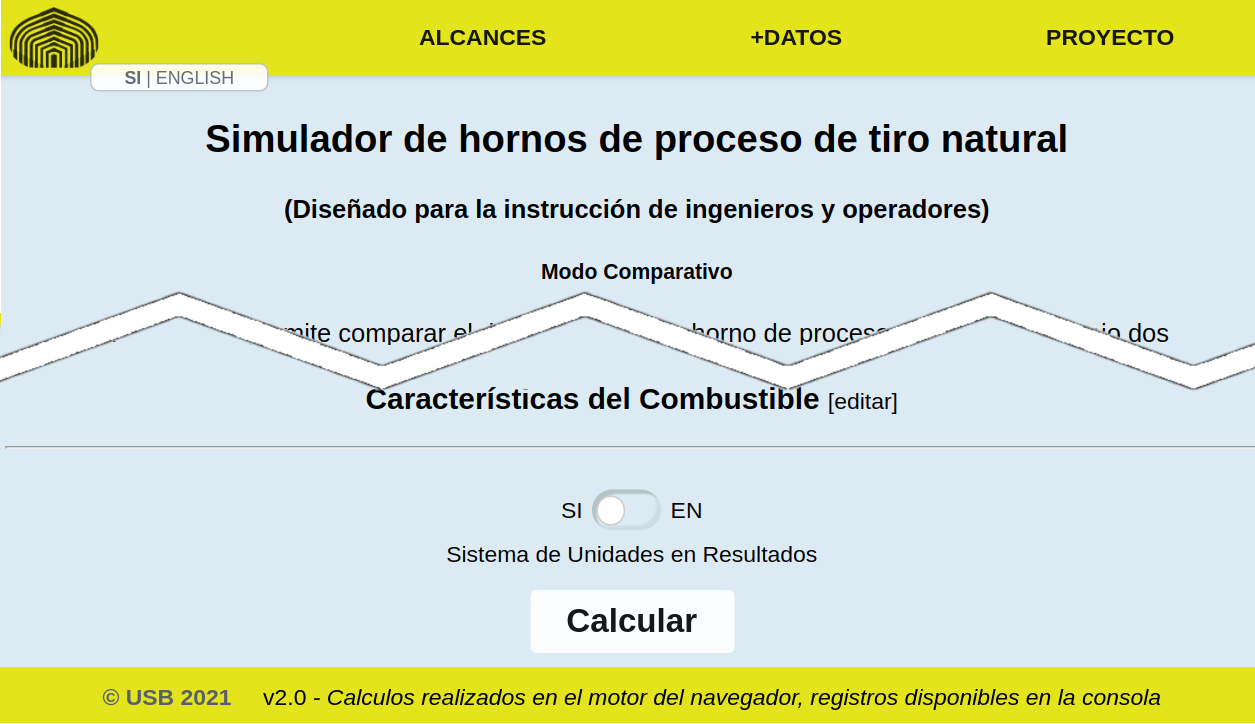
\includegraphics[scale=0.3]{images/datos}
\caption[Página de ingreso de datos para comparación]{Referencia a página de ingreso de datos utilizada para accionar el cálculo en la vista comparativa de resultados.}
\label{fig:datos}
\end{center}
\end{figure}
\begin{figure}[hbt]
\begin{center}
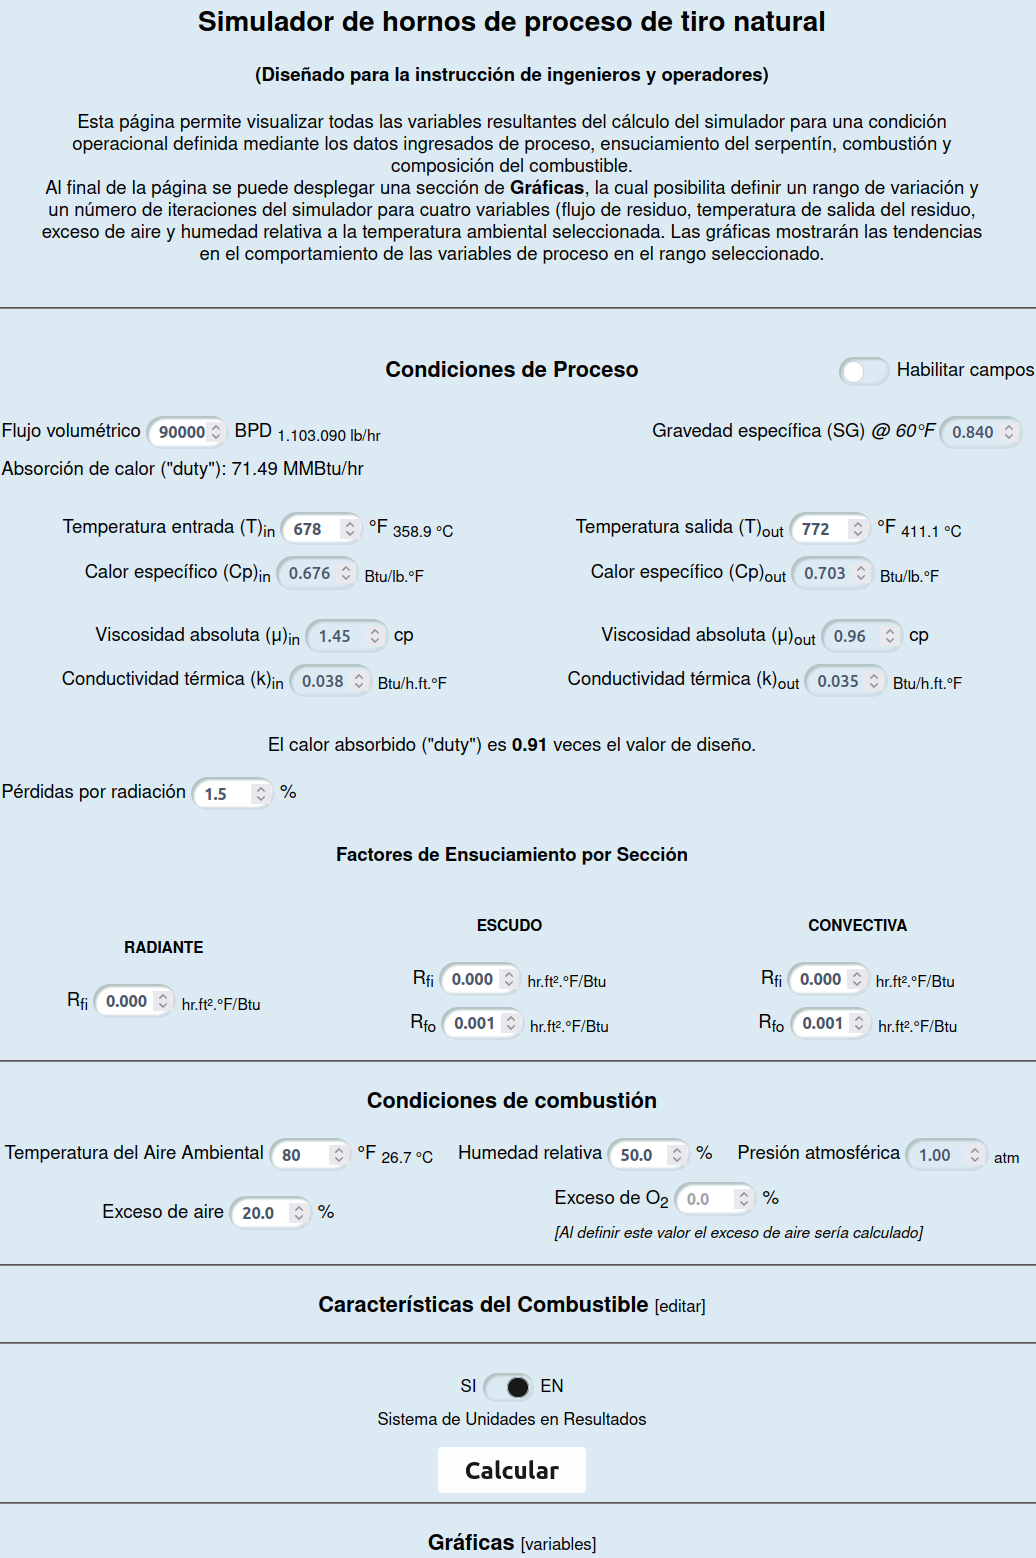
\includegraphics[scale=0.3]{images/datos2}
\caption[Página de ingreso de datos extendida]{Referencia a página de ingreso de datos extendida, con la opción de accionar la vista de resultados extendidos o la generación de gráficas de tendencia.}
\label{fig:fulldatos}
\end{center}
\end{figure}
\par En ambas se puede modificar la composición molar del combustible al pulsar la opción ``editar'', como se muestra en la Figura \ref{fig:edit_fuel}:
\begin{figure}[H]
\begin{center}

\includegraphics[scale=0.6]{images/edit_fuel}
\caption[Opción para editar el combustible]{Opción para editar el combustible al ingresar los datos.}
\label{fig:edit_fuel}
\end{center}
\par Un ejemplo de los campos abiertos para la edición de la composición del combustible se puede apreciar en la Figura \ref{fig:edit_fuel_ext}:
\end{figure}
\begin{figure}[hbt]
\begin{center}
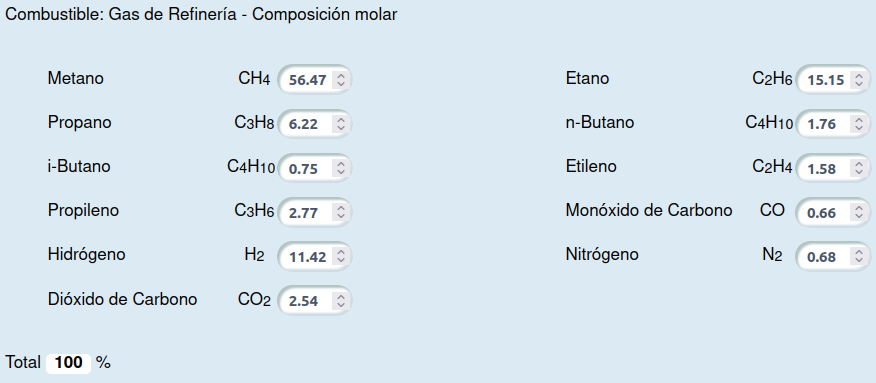
\includegraphics[scale=0.45]{images/edit_fuel_ext}
\caption[Campos para editar la composición del combustible]{Campos para editar la composición del combustible.}
\label{fig:edit_fuel_ext}
\end{center}
\end{figure}

\subsection{Resultados comparativos}
\par Esta vista es el resultado de accionar el cálculo en la sección de ingreso de datos simplificada. Posee el mayor potencial educativo, al resumir todas las variables resultantes y hacer una comparación entre dos condiciones de operación (Fig. \ref{fig:resultados}).
\par Aquí se pueden observar directamente los cambios en variables de interés, como los datos de ingreso, las emisiones de dióxido de carbono, el consumo de combustible, la distribución de calor dentro del horno, la temperatura de salida de los gases de combustión y la eficiencia térmica.
\par La recomendación para su uso es modificar solo una variable a la vez para su correcta interpretación.
\begin{figure}[H]
\begin{center}
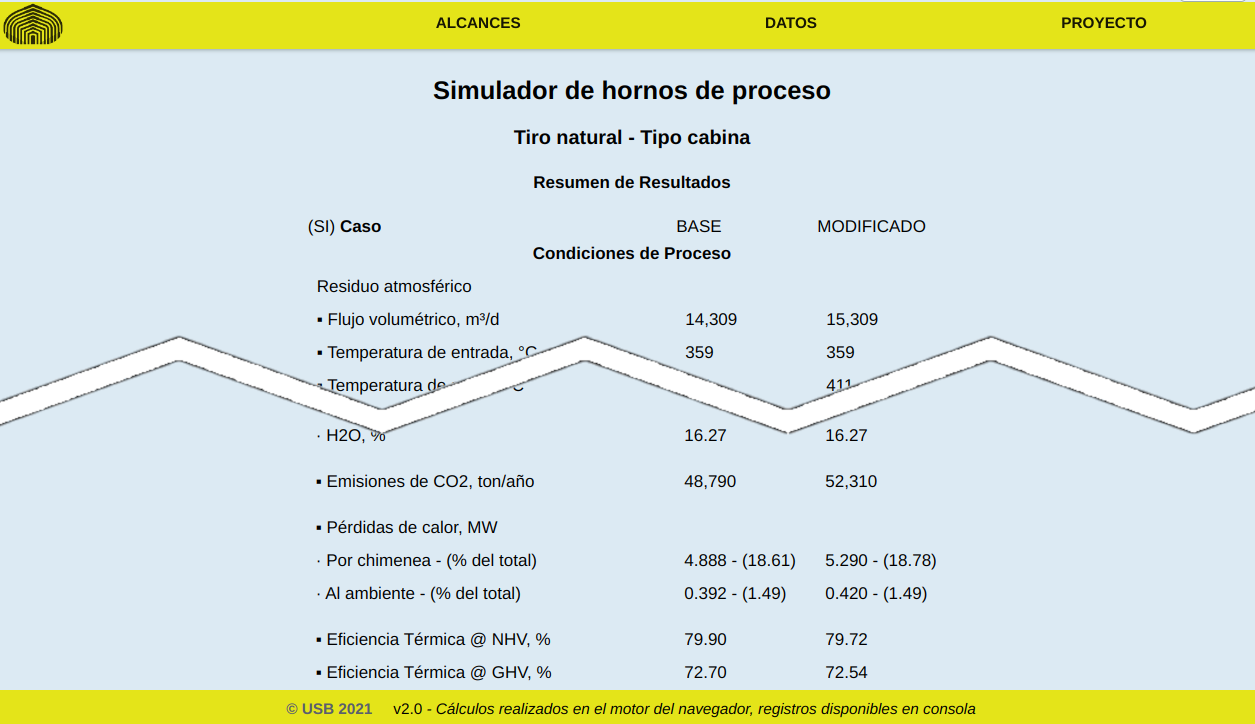
\includegraphics[scale=0.3]{images/result}
\caption[Página comparativa de resultados]{Referencia a página comparativa de resultados, donde se pueden detallar los cambios de un estado a otro en la operación del horno.}
\label{fig:resultados}
\end{center}
\end{figure}

\subsection{Resultados extendidos}
\par Esta vista es el resultado de accionar el cálculo en la sección de ingreso de datos extendidos. Aquí se detallan todas las variables resultantes por cada sección del horno (Fig. \ref{fig:fullresultados}), se puede escoger el sistema de unidades a expresarse en la pantalla anterior, se uso extensamente al depurar las ecuaciones internas del algoritmo para encontrar sus puntos críticos y corregirlos.
\par El objetivo de esta vista es tener una visión del comportamiento de todas las variables en el proceso, de aquí se pueden encontrar explicaciones no tan obvias del comportamiento de las variables finales mostradas en la vista comparativa.
\begin{figure}[H]
\begin{center}
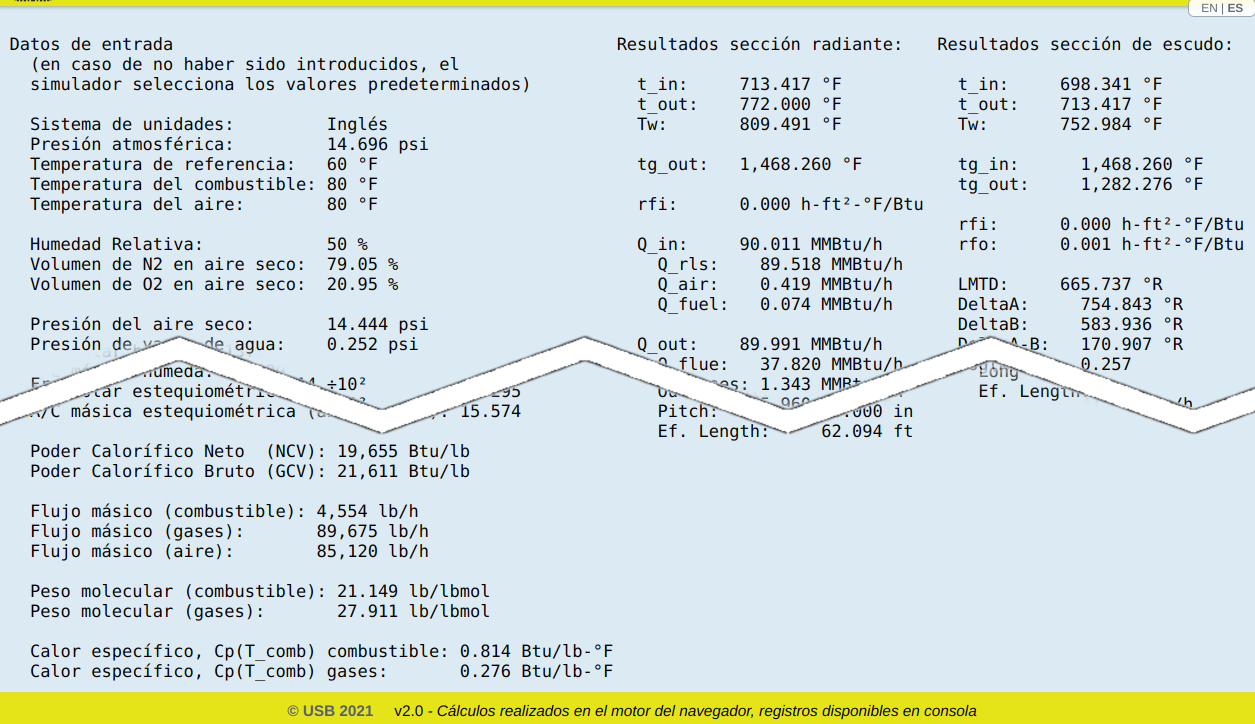
\includegraphics[scale=0.3]{images/result2}
\caption[Página extendida de resultados]{Referencia a página extendida de resultados, en ella se pueden observar a detalle las variables internas del proceso simulado.}
\label{fig:fullresultados}
\end{center}
\end{figure}

\subsection{Gráficas}
\par Esta página es pensada para los usuarios más curiosos, y para futuras modificaciones del algoritmo o extensión de sus rangos (ver Figura \ref{fig:graficas}).
\begin{figure}[H]\begin{center}
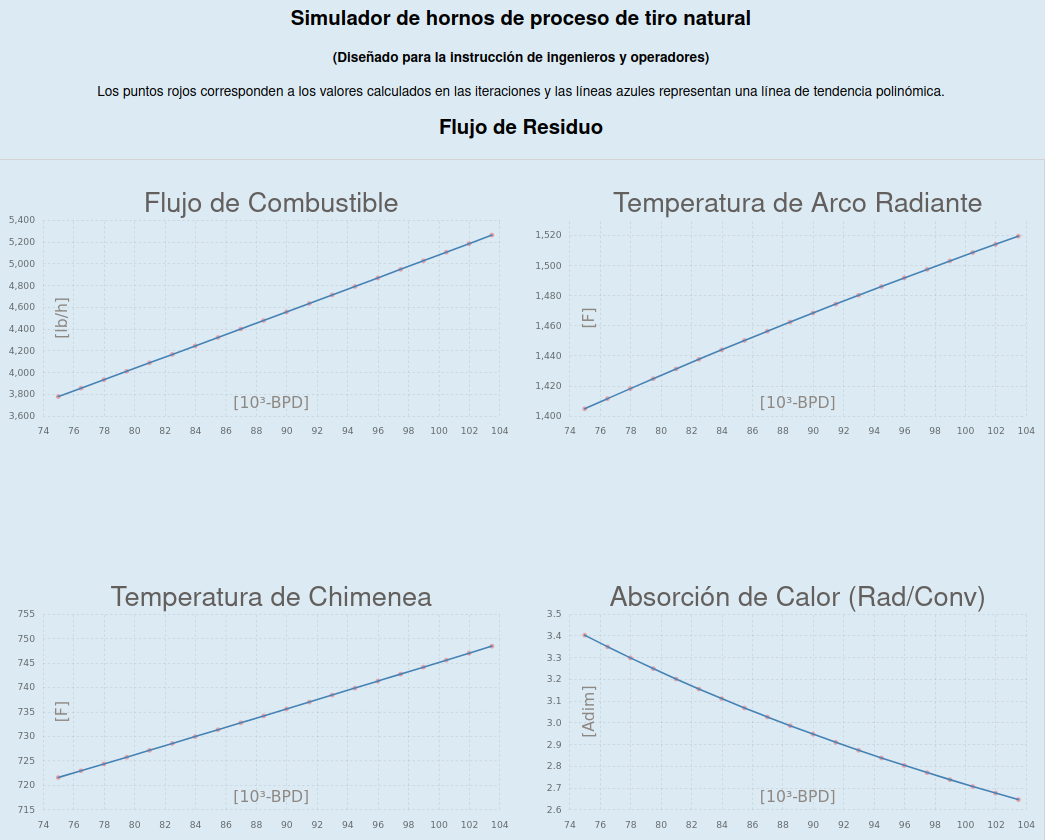
\includegraphics[scale=0.23]{images/graficas.png}
\caption[Página de gráficas]{Referencia de la página de gráficas, aquí se muestran las tendencias de las variables resultantes escogidas en el rango de variación determinado por el usuario.}
\label{fig:graficas} \end{center} \end{figure}
\par Para acceder a esta vista se debe accionar la opción de graficar ubicada al final de la página de ingreso de datos extendidos.
\par Su propósito es generar una visual del comportamiento del horno simulado a lo largo de un rango seleccionado, se usó para conseguir zonas donde los métodos aproximados del simulador no convergían y permitió sintonizar el paso, numero de iteraciones, valor inicial y tolerancia de dichos métodos.
\par Aquí se pueden comprobar las tendencias, la continuidad y la estabilidad de las variables resultantes; también facilita la comprensión de los resultados de los fenómenos dentro del horno.

\section{Despliegue del simulador en la web}
\par En el apartado ``PROYECTO'' de la barra de navegación en la interfaz, mostrado en la Figura \ref{fig:navbar}, se puede acceder al repositorio del proyecto, ubicado en GitHub, servidor que aloja el software del simulador y lo mantiene en línea.
\par GitHub es una plataforma de alojamiento de código para el control de versiones y la colaboración. Permite trabajar de forma individual o en equipos para desarrollar proyectos con acceso desde cualquier lugar con conexión a internet.
\par Adicionalmente permite publicar sitios web estáticos, que no requieran manejo de base de datos en la nube o procesamiento de datos a nivel del servidor, para proyectos de código abierto.
\par Se usó esta ventajosa función para hacer el simulador accesible desde cualquier navegador y se encuentra disponible en el siguiente enlace: \url{https://e-usb.github.io/heater}
\par Para acceder al código alojado en GitHub se puede seguir el mismo enlace ubicado en la pestaña ``PROYECTO'' de la interfaz del simulador. \url{https://github.com/e-usb/heater}